%=======================02-713 LaTeX template, following the 15-210 template==================
%
% You don't need to this template
%
\documentclass[11pt]{article}
\usepackage{amsmath,amssymb,amsthm}
\usepackage{graphicx}
\usepackage{wrapfig}
\usepackage[margin=1in]{geometry}
\usepackage{fancyhdr}
\setlength{\parindent}{0pt}
\setlength{\parskip}{5pt plus 1pt}
\setlength{\headheight}{13.6pt}
\newcommand\question[2]{\vspace{.25in}\hrule\textbf{#1: #2}\vspace{.5em}\hrule\vspace{.10in}}
\renewcommand\part[1]{\vspace{.10in}\textbf{(#1)}}
\newcommand\algorithm{\vspace{.10in}\textbf{Algorithm: }}
\newcommand\correctness{\vspace{.10in}\textbf{Correctness: }}
\newcommand\runtime{\vspace{.10in}\textbf{Running time: }}
\newcommand\tab[1][1cm]{\hspace*{#1}}
\pagestyle{fancyplain}
\lhead{\textbf{\NAME\ (\ANDREWID)}}
\chead{\textbf{HW\HWNUM}}
\rhead{02-713, \today}
\begin{document}\raggedright
%Section A==============Change the values below to match your information==================
\newcommand\NAME{Kadir Emre Otod}  % your name
\newcommand\ANDREWID{150140032}     % your andrew id
\newcommand\HWNUM{3}              % the homework number
%Section B==============Put your answers to the questions below here=======================

% no need to restate the problem --- the graders know which problem is which,
% but replacing "The First Problem" with a short phrase will help you remember
% which problem this is when you read over your homeworks to study.

\question{1}{Casuality and Stability} 

\part{a} \\
\tab \textbf{Not casual:} The function is dependent on future \\
\tab \textbf{Stable:} x and y can be bounded.

\part{b} \\
\tab \textbf{Casual:} The function is independent on future \\
\tab \textbf{Not stable:} x and y cannot be bounded.

\part{c} \\
\tab \textbf{Casual:} The function is independent on future \\
\tab \textbf{Stable:} The function cannot exceed 1.

\part{d} \\
\tab \textbf{Casual:} The function is independent on future \\
\tab \textbf{Stable:} The function cannot exceed 1.


\question{2}{Convolution} 

\begin{eqnarray*}
	h(t) &=& 5e ^ {-0.5(t-3)} [u(t-3) - u(t-11)] \\
	x(t) &=& u(t-2) \\
	y[n] &=& \sum_{k=-\infty}^{\infty} h[k] [n-k] \\
	&=& \sum_{k=-\infty}^{\infty} 5e ^ {-0.5(k-3)} [u(k-3) - u(k-11)]  u(n-2-k)
\end{eqnarray*}

\cleardoublepage

\question{3}{FFT Implementation} 

\begin{figure}[h]
	\centering
	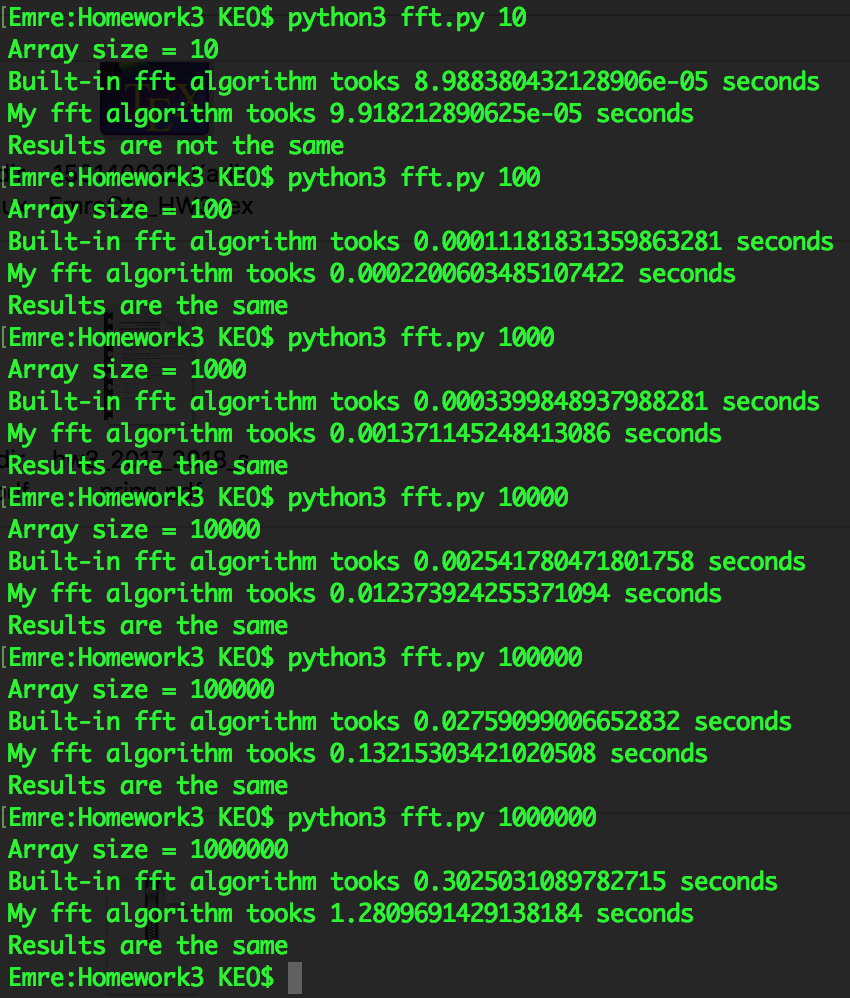
\includegraphics[width=0.7\linewidth]{results}
	\caption{The compare results of fft algorithms}
	\label{fig:results}
\end{figure}

\cleardoublepage

\question{4}{Convolution} 

\begin{figure}[h]
	\centering
	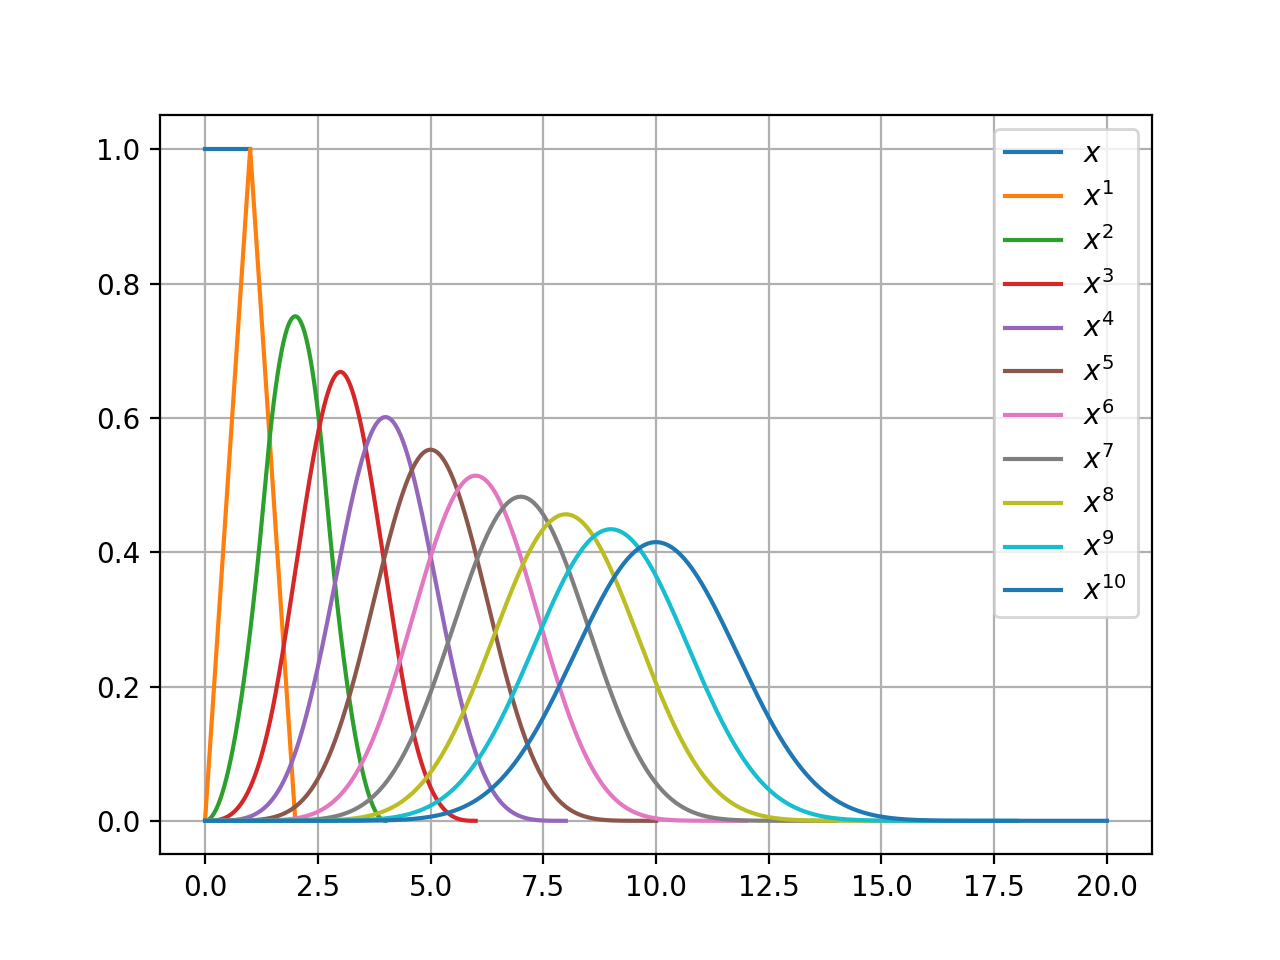
\includegraphics[width=0.7\linewidth]{convolution}
	\caption{The graph of convolution result}
	\label{fig:convolution}
\end{figure}

\cleardoublepage

\question{5}{Frequency Response and Superposition} 

\part{a} \\
\begin{eqnarray*}
	H(jw) &=& \int\limits_{-\infty}^{\infty} h(t) e^{-jwt} dt \\
	H(jw) &=& \int\limits_{-\infty}^{\infty} (\delta(t-2)-0.2e^{-0.2(t-2)}[u(t-2)]) e^{-jwt} dt \\
	&=& \int\limits_{-\infty}^{\infty} \delta(t-2) e^{-jwt} dt +  \int\limits_{-\infty}^{\infty} -0.2e^{-0.2(t-2)}[u(t-2)] e^{-jwt} dt \\
	&=& e^{-2jw} - 0.2e^{0.4} \int\limits_{2}^{\infty} e ^{-(0.2+jw)t} dt \\
	&=& e^{-2jw} + 0.2e^{0.4}\dfrac{e^{-(0.4 + 2jw)}}{-(0.2 + jw)} \\
	&=& e^{-2jw} - \dfrac{0.2e^{-2jw}}{0.2 + jw}\\
	&=& \dfrac{jwe^{-2jw}}{0.2 + jw}
\end{eqnarray*}

\part{b} \\


\part{c} \\
\begin{eqnarray*}
	x_1(t) &=& 5, \tab x_2(t) = 10cos(0.2t), \tab x_3(t)=u(t) \\
	y_1(t) &=& H(j0) = 0 \\
	y_2(t) &=& 10 \dfrac{e^{-0.4j}}{\sqrt{2}}cos(0.2t+\dfrac{\pi}{4}) \\
	y_3(t) &=& u(t) \cdot h(t) \\
	&=& u(t-2) +  \int\limits_{2}^{\infty} -0.2 e ^{-0.2(t-2)} u(t-2)u(\tau-t) dt \\
	&=& u(t-2)(1-0.2e^{0.4}(t-2)) \\
	y(t) &=& 10 \dfrac{e^{-0.4j}}{\sqrt{2}}cos(0.2t+\dfrac{\pi}{4}) + u(t-2)(1-0.2e^{0.4}(t-2)) \\
\end{eqnarray*}

\cleardoublepage

\question{6}{Fourier Transforms} 

\part{a} \\

\begin{eqnarray*}
	\dfrac{1}{2 \pi} \int\limits_{-\infty}^{\infty} \dfrac{sin^2(10w)}{2w^2} e^{jwt} dw
\end{eqnarray*}

\part{b} \\

\begin{eqnarray*}
	\dfrac{1}{2 \pi} \int\limits_{-\infty}^{\infty} \dfrac{1}{25 + w^2} e^{jwt} dw
\end{eqnarray*}

\part{c} \\

\begin{eqnarray*}
	\dfrac{1}{2 \pi} \int\limits_{-\infty}^{\infty} e^{-a(t-2)}u(t-2)cos(w_0t)e^{-jwt} dt \\
	= \dfrac{1}{2 \pi} \int\limits_{2}^{\infty} e^{-a(t-2)}cos(w_0t)e^{-jwt} dt
\end{eqnarray*}

\question{7}{} 

\tab \\
\tab \\
\tab \\
\tab \\
\tab \\
\tab \\





\end{document}
